\documentclass{eh-homework}

\begin{document}
\usetikzlibrary{arrows.meta}
\section*{Assignment 3: Due March 16, 2025 (Sunday) at 11:59PM ET}

Answers must be submitted via Crowdmark using your personalized submission link (which will be sent to your email). Late submissions will not be accepted.

If you used Octave to assist you in solving a problem, also attach to the solution to that problem the script and commands you used and the corresponding outputs obtained.

A proper selection of questions from the ones below will be graded.

\begin{question}{1}
\textbf{(5.1, \#18)} The Bézier curve
\[
x(t) = 11t^3 - 18t^2 + 3t + 5
\]
\[
y(t) = t^3 + 1
\]
has control points \((5,1)\), \((6,1)\), and \((1,2)\). Find the fourth control point.
\end{question}

\begin{question}{2}
Sketch a stencil for the following data, picking appropriate \(x_0\) and \(h\), that can be used to approximate \(f'(1)\). You do not need to derive the formula.

\[
\begin{array}{c|cccc}
x & -3 & -1.5 & 0 & 2 \\
\hline
f(x) & 3.11 & 3.05 & 3.4 & 3.7 \\
\end{array}
\]
\end{question}

\begin{question}{3}
\textbf{(4.1, \#13c)} Derive an approximation formula for the second derivative \( f'' \) over the stencil:

\begin{center}
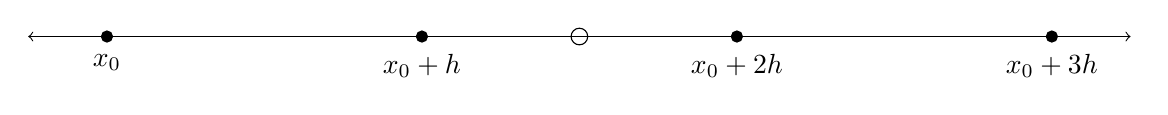
\begin{tikzpicture}
    \draw[<->] (-7,0) -- (7,0) node[below]{};
    \foreach \x/\label in {-6/\(x_0\), -2/\(x_0 + h\), 2/\(x_0 + 2h\), 6/\(x_0 + 3h\)} {
        \draw[fill] (\x, 0) circle (2pt);
        \node[below] at (\x,-0.1) {\label};
    }
    \draw (0, 0) circle (3pt);
\end{tikzpicture}
\end{center}

using a direct method as discussed in Section 4.1.
\end{question}

\begin{question}{4}
\textbf{(4.2, \#3c)} Over the same stencil as in the previous question, derive an approximation formula for the second derivative \( f'' \) but now using undetermined coefficients.
\end{question}

\begin{question}{5}
\textbf{(Based on 4.1, \#19)} Let \( x_0, x_0 + \alpha h, x_0 + 2h \) be nodes where \( \alpha \neq 0,2 \).

\begin{enumerate}[label=\alph*.]
    \item Write the first Taylor polynomials of \( f(x_0 +\alpha h) \) and \( f(x_0 +2h) \) around \( x = x_0 \), then use these to show that:
    \[
    f'(x_0) = \frac{1}{2h} \left[ \frac{-2+\alpha}{\alpha} f(x_0) + \frac{4}{\alpha(2-\alpha)} f(x_0 + \alpha h) - \frac{\alpha}{2-\alpha} f(x_0 + 2h) \right].
    \]

    \item Now show that the same result is obtained when using the method of undetermined coefficients.
\end{enumerate}
\end{question}

\begin{question}{6}
\textbf{(4.2, \#4i)} Use undetermined coefficients to derive an approximation formula for the integral over the stencil:

\begin{center}
\begin{tikzpicture}
    \draw[<->] (-1,0) -- (7,0);
    \draw[{Bracket[width=3mm]}-{Bracket[width=3mm]}] (0, 0) -- (6,0);
    \foreach \x/\label in {0/\(x_0\), 4/\(x_0 + \frac{4}{3}h\), 6/\(x_0 + 2h\)} {
        \draw[fill] (\x, 0) circle (2pt);
        \node[below] at (\x,-0.1) {\label};
    }

\end{tikzpicture}
\end{center}

\end{question}

\vfill
\centerline{End of Assignment 3}

\end{document}